\documentclass[10pt,twocolumn]{article}
\usepackage[margin=0.72in]{geometry}
\usepackage{amsmath,amssymb,amsthm,graphicx,microtype,url,algorithm,algorithmic}
\usepackage[hidelinks]{hyperref}
\newtheorem{proposition}{Proposition}
\newtheorem{lemma}{Lemma}
\newcommand{\method}{Multi-Back Flow}
\title{Multi-Back Flow:\\Optimization-Guided Flow Maps for Inverse Problems}
\author{Haoyang Jiang\\William \& Mary}
\date{}

\begin{document}
\maketitle

\begin{abstract}
Pretrained generative models provide reusable priors for inverse problems, but conditioning them on a new measurement operator remains challenging. Supervised inverse networks offer fast inference yet couple the reconstruction rule to operators and acquisition settings represented during training; under multimodal ambiguity, pointwise regression can further favor conditional averages. Diffusion posterior methods avoid task-specific retraining by introducing measurement information at inference time, but often require long denoising chains or repeated posterior refinement. Optimization-Guided Diffusion (OGD) instead optimizes controls along a frozen DDIM trajectory.

We introduce \method{} (MBF), which extends optimization-guided generation from a fixed denoising chain to a non-monotone trajectory built from a frozen two-time Flow Map. Flow maps enable few-step generation through long temporal transitions, but a few-step monotone path exposes only a small number of control locations and can become locally locked when the task gradient is poorly represented by its endpoint control Jacobian. MBF inserts controlled backward--forward transitions to earlier generative times, where additional controls open endpoint directions unavailable to the monotone parameterization. The general trajectory objective contains generative-source, monotone, and Back controls, while the reported FWI solver uses a staged source-then-Multi-Back schedule. We provide a local descent characterization of basin lock and show how Multi-Back controls restore first-order descent directions. A synthetic full-waveform inversion study demonstrates the current implementation; broader validation across operators and domains remains future work.
\end{abstract}

\section{Introduction}
Inverse problems seek to recover an unknown object $x$ from incomplete, noisy, or indirect observations $y$. A useful reconstruction must satisfy both measurement consistency and structural plausibility. Supervised deterministic inverse networks, including U-Net-style encoder--decoders and InversionNet, directly learn $f_\theta:y\mapsto x$ from paired data and provide fast inference \cite{ronneberger2015unet,wu2019inversionnet}. Their reconstruction rule, however, is tied to the observation distributions and acquisition configurations represented during training. Under squared error, the population-optimal deterministic predictor is $f^\star(y)=\mathbb E[x\mid y]$; when one observation is compatible with multiple sharp solutions, this conditional average can blur or superpose distinct modes \cite{blau2018perception}. Neural operators such as FNO learn mappings between function spaces and amortize repeated solves over a parameterized operator family, but inverse use still depends on the operators, parameter ranges, and discretizations covered by training \cite{li2021fno}. Conditional generative models such as pix2pix and VelocityGAN can encourage sharper outputs, yet their conditioning interfaces remain tied to paired task-specific data \cite{isola2017pix2pix,zhang2019velocitygan}.

Pretrained unconditional generative models provide a more modular alternative: the model learns a prior over solutions, while a new measurement operator enters only at inference time. Diffusion-based inverse methods have pursued this idea through analytic linear methods, manifold- or likelihood-guided methods such as MCG, DPS, and $\Pi$GDM, and optimization or resampling methods that impose stronger data consistency \cite{chung2022mcg,chung2023dps,song2023pigdm,zhu2023diffpir,song2024resample}. These approaches broaden the reuse of a frozen prior, but commonly require repeated denoiser evaluations, forward-operator calls, or inner refinement across many noise levels. DAPS explicitly identifies the difficulty of correcting early global errors and decouples consecutive noise levels through clean-space posterior sampling followed by fresh-noise annealing \cite{zhang2025daps}.

OGD offers a complementary optimization view: it replaces perturbations along a fixed DDIM trajectory with optimized controls, turning inference into constrained trajectory optimization while keeping the generator frozen \cite{ogd2026}. This is a natural starting point for general inverse and constrained-generation problems, but its controls remain attached to a prescribed monotone denoising chain. Flow Map Matching learns the two-time transport map of an underlying generative dynamics and supports long transitions between arbitrary generative times, enabling one- or few-step generation with a post-training choice of step count \cite{boffi2024flowmap}. Replacing DDIM transitions with Flow Map transitions reduces generative cost, but it does not remove the restriction to a monotone source-to-data path.

Few-step optimization makes this restriction especially important. For a schedule $1=t_0>\cdots>t_K=0$, at least one transition spans $1/K$ or more in generative time, while only $K$ locations are available for ordinary controls. An early control can therefore strongly determine the basin reached by the remaining path. Near a locally restricted endpoint, the task gradient may have only a weak projection onto the endpoint directions generated by monotone controls, producing \emph{few-step basin lock}. We propose \method{} to address this failure mode. MBF treats generative time as a bidirectional optimization coordinate: it returns a trajectory state to an earlier generative time, applies a task-driven Back control, and transports the controlled state forward again.

Conceptually, MBF extends optimization-guided generation from control on a fixed chain to non-monotone control on a two-time flow graph. Unlike posterior re-noising, restart sampling, or DAPS-style annealing, MBF does not draw a fresh noisy posterior state; the backward--forward transition is part of a deterministic controlled trajectory. Our contributions are an optimization-guided formulation for few-step Flow Maps, a local characterization of basin lock, Multi-Back temporal recourse that adds endpoint directions from earlier generative scales, and a staged FWI realization separating global source selection from later recourse.

\section{Preliminaries}
\subsection{Inverse problems with frozen generative priors}
We consider $y=\mathcal A(x^\star)+\eta$, where $x^\star\in\mathcal X$ is unknown, $\mathcal A:\mathcal X\to\mathcal Y$ is known, and $\eta$ is measurement noise. A task loss $\mathcal L_y(x)=\ell(\mathcal A(x),y)$ measures consistency; for Gaussian noise, $\mathcal L_y(x)=\|\mathcal A(x)-y\|^2/(2\sigma_y^2)$. Additional constraints may be written as $g_j(x)\le0$ and $h_\ell(x)=0$. The generative prior is pretrained independently of $\mathcal A$ and remains frozen during inference.

\subsection{Optimization-Guided Diffusion}
A stochastic DDIM transition can be written schematically as $x_{k-1}=\mu_\theta(x_k,k)+\sigma_k\omega_k$, with $\omega_k\sim\mathcal N(0,I)$. OGD replaces $\omega_k$ with an optimized correction $\delta_k$ and solves
\begin{equation}
\min_{x_K,\{\delta_k\}}\;\mathcal L_y(x_0)+\frac{\lambda_K}{2}\|x_K\|^2+\frac12\sum_{k=1}^K\lambda_k\|\delta_k\|^2,
\quad x_{k-1}=\mu_\theta(x_k,k)+\sigma_k\delta_k.
\end{equation}
MBF inherits this control-space view but replaces the fixed DDIM chain with a two-time Flow Map and augments the monotone path with temporal recourse.

\subsection{Two-time Flow Maps}
Let $\Phi_\theta(\cdot;r,t):\mathcal X_r\to\mathcal X_t$ denote a learned two-time Flow Map, abbreviated as $\Phi_{t\leftarrow r}$. For $1=t_0>\cdots>t_K=0$, few-step generation uses $z_{t_{i+1}}=\Phi_{t_{i+1}\leftarrow t_i}(z_{t_i})$. A learned Flow Map directly provides long temporal transitions and permits the number of sampling steps to be selected after training \cite{boffi2024flowmap}. Its two-time interface also permits mappings toward earlier generative times, which MBF uses as optimization coordinates rather than fresh-noise resampling operations.

\section{Multi-Back Flow}
MBF distinguishes a generative source control at $t=1$ from controls inserted along or behind an established trajectory. The source control can change the full coarse trajectory and therefore the reconstruction basin; Back controls provide recourse after a source trajectory has been formed.

\subsection{Generative source and controlled monotone Flow Maps}
Given $1=t_0>\cdots>t_K=0$ and $\xi\sim p_{\mathrm{src}}$, the initial generative state is
\begin{equation}
z_{t_0}=\xi+B_{\mathrm{src}}a,
\end{equation}
where $a$ is a source displacement. Here \emph{source} refers to the generative source at $t=1$, not the physical seismic source $s(\mathbf r,t)$ in the acoustic wave equation. Changing $a$ changes every downstream Flow Map state and may therefore select a different coarse reconstruction basin. Ordinary controls are injected as
\begin{equation}
z_{t_{i+1}}=\Phi_{t_{i+1}\leftarrow t_i}(z_{t_i}+B_i u_i),\qquad i=0,\ldots,K-1.
\end{equation}
Writing $c=(a,u_0,\ldots,u_{K-1})$, the endpoint is $x_{\mathrm{mono}}(c)=\mathcal G_{\mathrm{mono}}(\xi;c)$. The monotone objective is
\begin{equation}
\min_c\;\mathcal L_y(x_{\mathrm{mono}}(c))+\frac{\lambda_{\mathrm{src}}}{2}\|a\|^2+\frac12\sum_{i=0}^{K-1}\lambda_i\|u_i\|^2.
\end{equation}

\subsection{Few-step basin lock}
Let $\Delta t_i=t_i-t_{i+1}$. Since $\sum_i\Delta t_i=1$, $\max_i\Delta t_i\ge1/K$. At $x=x_{\mathrm{mono}}(c)$, let $g=\nabla_x\mathcal L_y(x)$ and $J_{\mathrm{mono}}=D_c\mathcal G_{\mathrm{mono}}(\xi;c)$. Under $\|\delta c\|\le\epsilon$, the maximum first-order decrease equals $\epsilon\|J_{\mathrm{mono}}^\top g\|$.

\begin{proposition}[Local basin-lock criterion]
If $J_{\mathrm{mono}}^\top g=0$, no sufficiently small monotone-control update decreases the task loss to first order. More generally, a small ratio $\|J_{\mathrm{mono}}^\top g\|/\|g\|$ indicates that the task gradient is poorly represented by the endpoint directions available to the monotone parameterization.
\end{proposition}

\subsection{Multi-Back temporal recourse}
For a state $z_\tau$ and an earlier, higher-noise time $\rho$ with $0\le\tau<\rho\le1$, a Back module is
\begin{equation}
\mathcal B_{\tau,\rho}(z_\tau;b)=\Phi_{\tau\leftarrow\rho}\!\left(\Phi_{\rho\leftarrow\tau}(z_\tau)+C b\right).
\end{equation}
For $M$ modules, let $\Gamma=\{(\tau_m,\rho_m)\}_{m=1}^M$ and $b=(b_1,\ldots,b_M)$. Inserting these events yields $x_{\mathrm{MBF}}(c,b;\Gamma)=\mathcal G_{\mathrm{MBF}}(\xi;c,b,\Gamma)$.

Let $J_c=D_cx_{\mathrm{MBF}}$ and $J_b=D_bx_{\mathrm{MBF}}$. Under $\|[\delta c;\delta b]\|\le\epsilon$, the maximum first-order decrease is $\epsilon\sqrt{\|J_c^\top g\|^2+\|J_b^\top g\|^2}$.

\begin{proposition}[Local unlocking]
If $J_c^\top g=0$ but $J_b^\top g\ne0$, ordinary monotone controls provide no first-order descent direction, whereas the Multi-Back parameterization does.
\end{proposition}

\subsection{Trajectory objective and staged FWI schedule}
The variables belong to one trajectory objective,
\begin{equation}
\min_{a,\{u_i\},\{b_m\}}\;\mathcal L_y(x_{\mathrm{MBF}})+\frac{\lambda_{\mathrm{src}}}{2}\|a\|^2+\frac12\sum_i\lambda_i\|u_i\|^2+\frac12\sum_m\gamma_m\|b_m\|^2.
\end{equation}
They need not be updated simultaneously. The reported FWI solver first optimizes the generative source through a coarse-to-fine measurement objective. This stage chooses a measurement-informed global trajectory and supplies the intermediate state $z_\tau$ at the prespecified time $\tau$, where the first Multi-Back correction is introduced. The solver then holds that source fixed and optimizes Multi-Back controls, which revisit earlier generative times to provide recourse and refinement around the established trajectory. The staged schedule separates a global basin-setting coordinate from later recourse coordinates and serves as an optimization warm start; it is not an assumption that source and Back controls are mathematically independent.

\begin{algorithm}[t]
\caption{Staged Multi-Back Flow}
\begin{algorithmic}[1]
\STATE Sample $\xi\sim p_{\mathrm{src}}$ and initialize $a\leftarrow0$.
\STATE Optimize $a$ through the source-to-data trajectory.
\STATE Construct $z_\tau$ from the optimized source at the prespecified time $\tau$.
\STATE Insert Back modules according to $\Gamma$.
\STATE Optimize monotone and Back controls with the source fixed.
\RETURN The final endpoint.
\end{algorithmic}
\end{algorithm}

\section{FWI Case Study}
We use a frozen optimal-transport FlowMap trained as an unconditional $70\times70$ geological prior. A differentiable acoustic forward model maps the endpoint to receiver observations. Classical FWI is a nonconvex wave-equation data-fitting problem \cite{virieux2009fwi}; InversionNet is a representative task-trained CNN alternative \cite{wu2019inversionnet}. Five evaluation rows (29864, 29748, 29544, 29952, 29694) are crossed with raw seeds 20268032--20268432. The algorithm, grid, action budget, and hashes were recorded in a frozen manifest before the remaining panel was run. Truth is opened only after each endpoint record is frozen and is used for post-decision MSE and boundary F1.

FWI-specific acquisition, checkpoint, split, exposure-history, and metric details are separated into the \href{../docs/fwi_appendix.md}{archival appendix}, keeping the main formulation task-agnostic.

\subsection{Baseline comparison with row-oracle ours}
\begin{figure}[t]
\centering
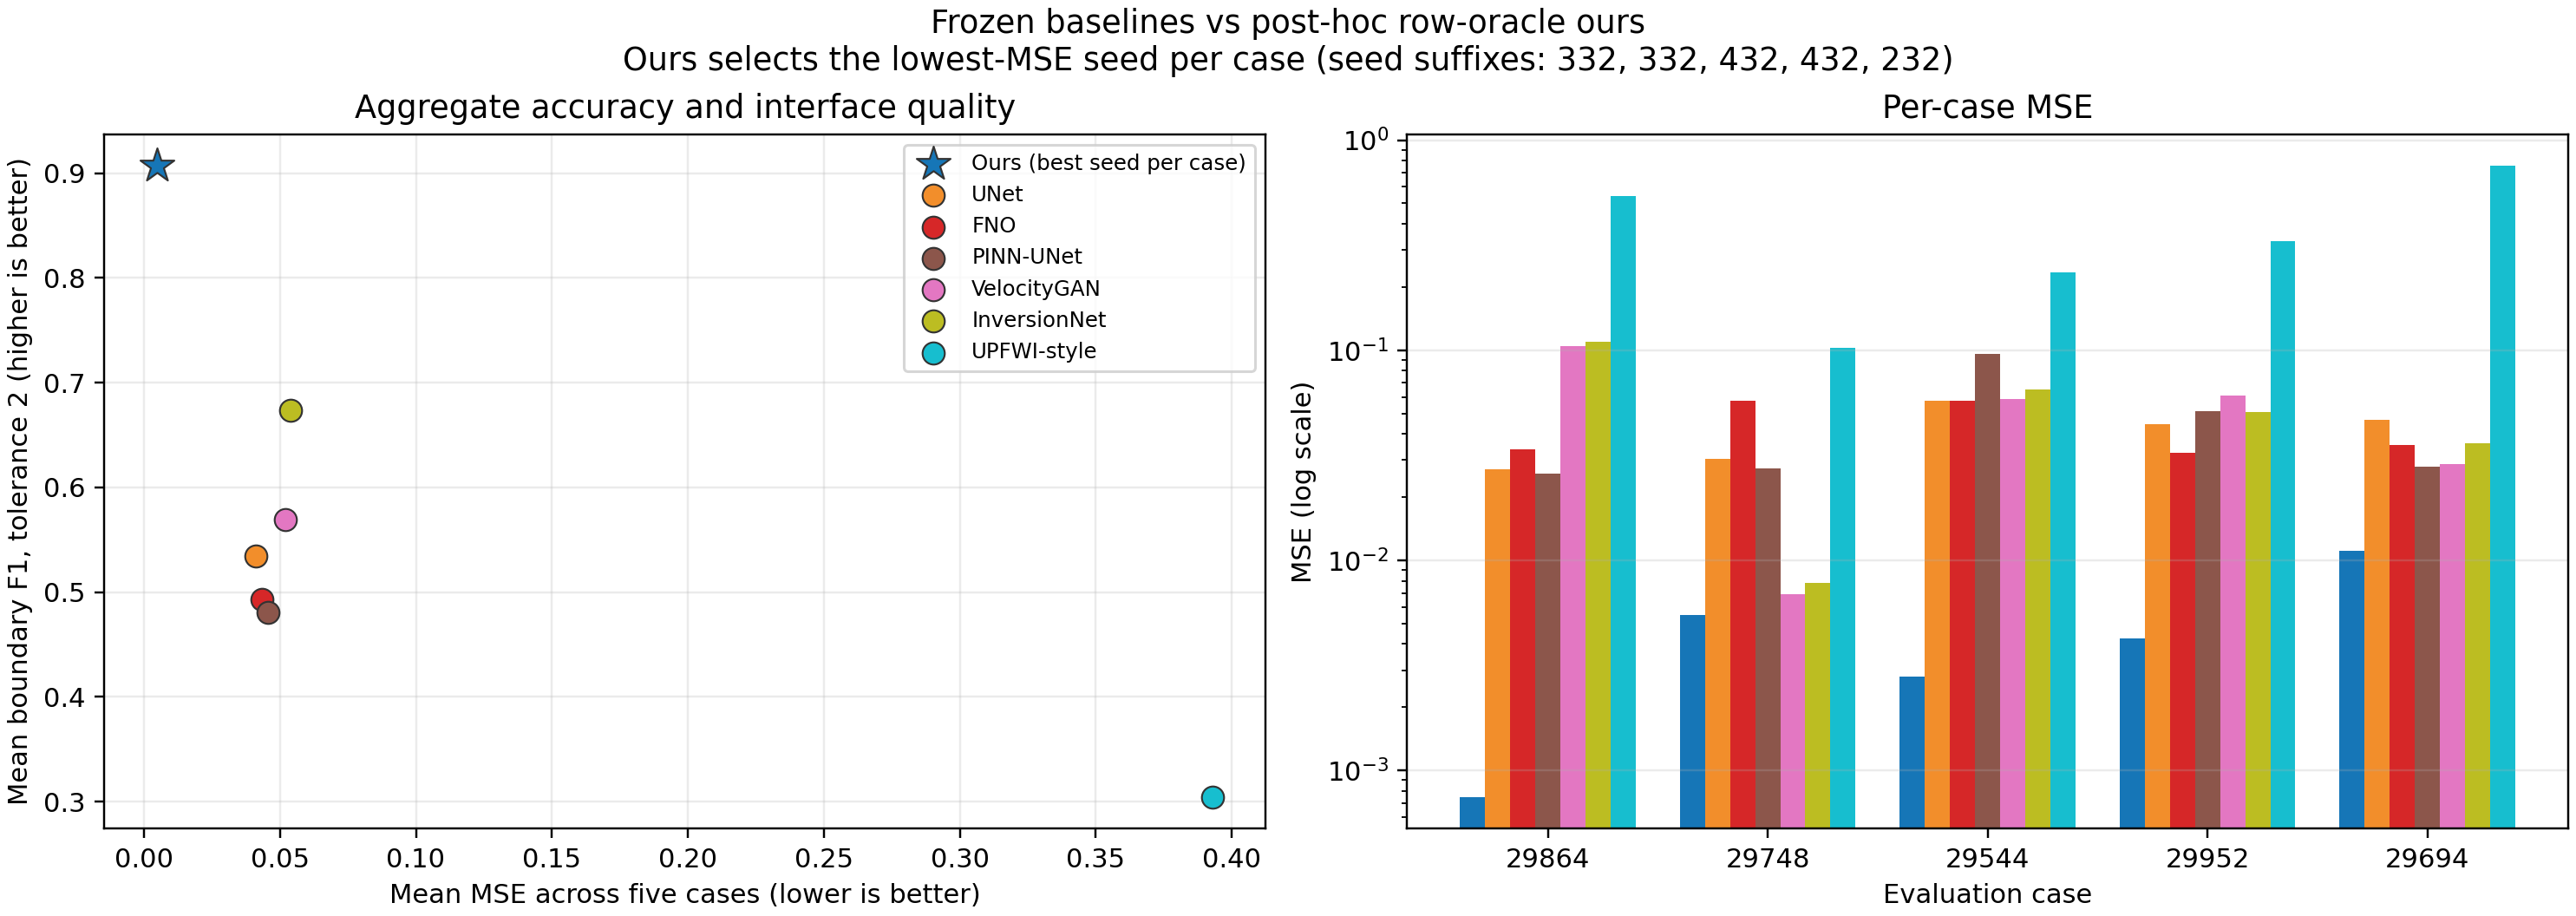
\includegraphics[width=\columnwidth]{../assets/figures/method_comparison.png}
\caption{Frozen task-trained baselines versus ours with the lowest-MSE seed selected separately for each evaluation case. The selected seed suffixes are 332, 332, 432, 432, and 232 in row order. This is a post-hoc row-oracle visualization using truth MSE, not an inference-time selection rule or a compute-matched superiority claim.}
\label{fig:comparison}
\end{figure}

\subsection{Five cases $\times$ five seeds}
\begin{figure}[t]
\centering
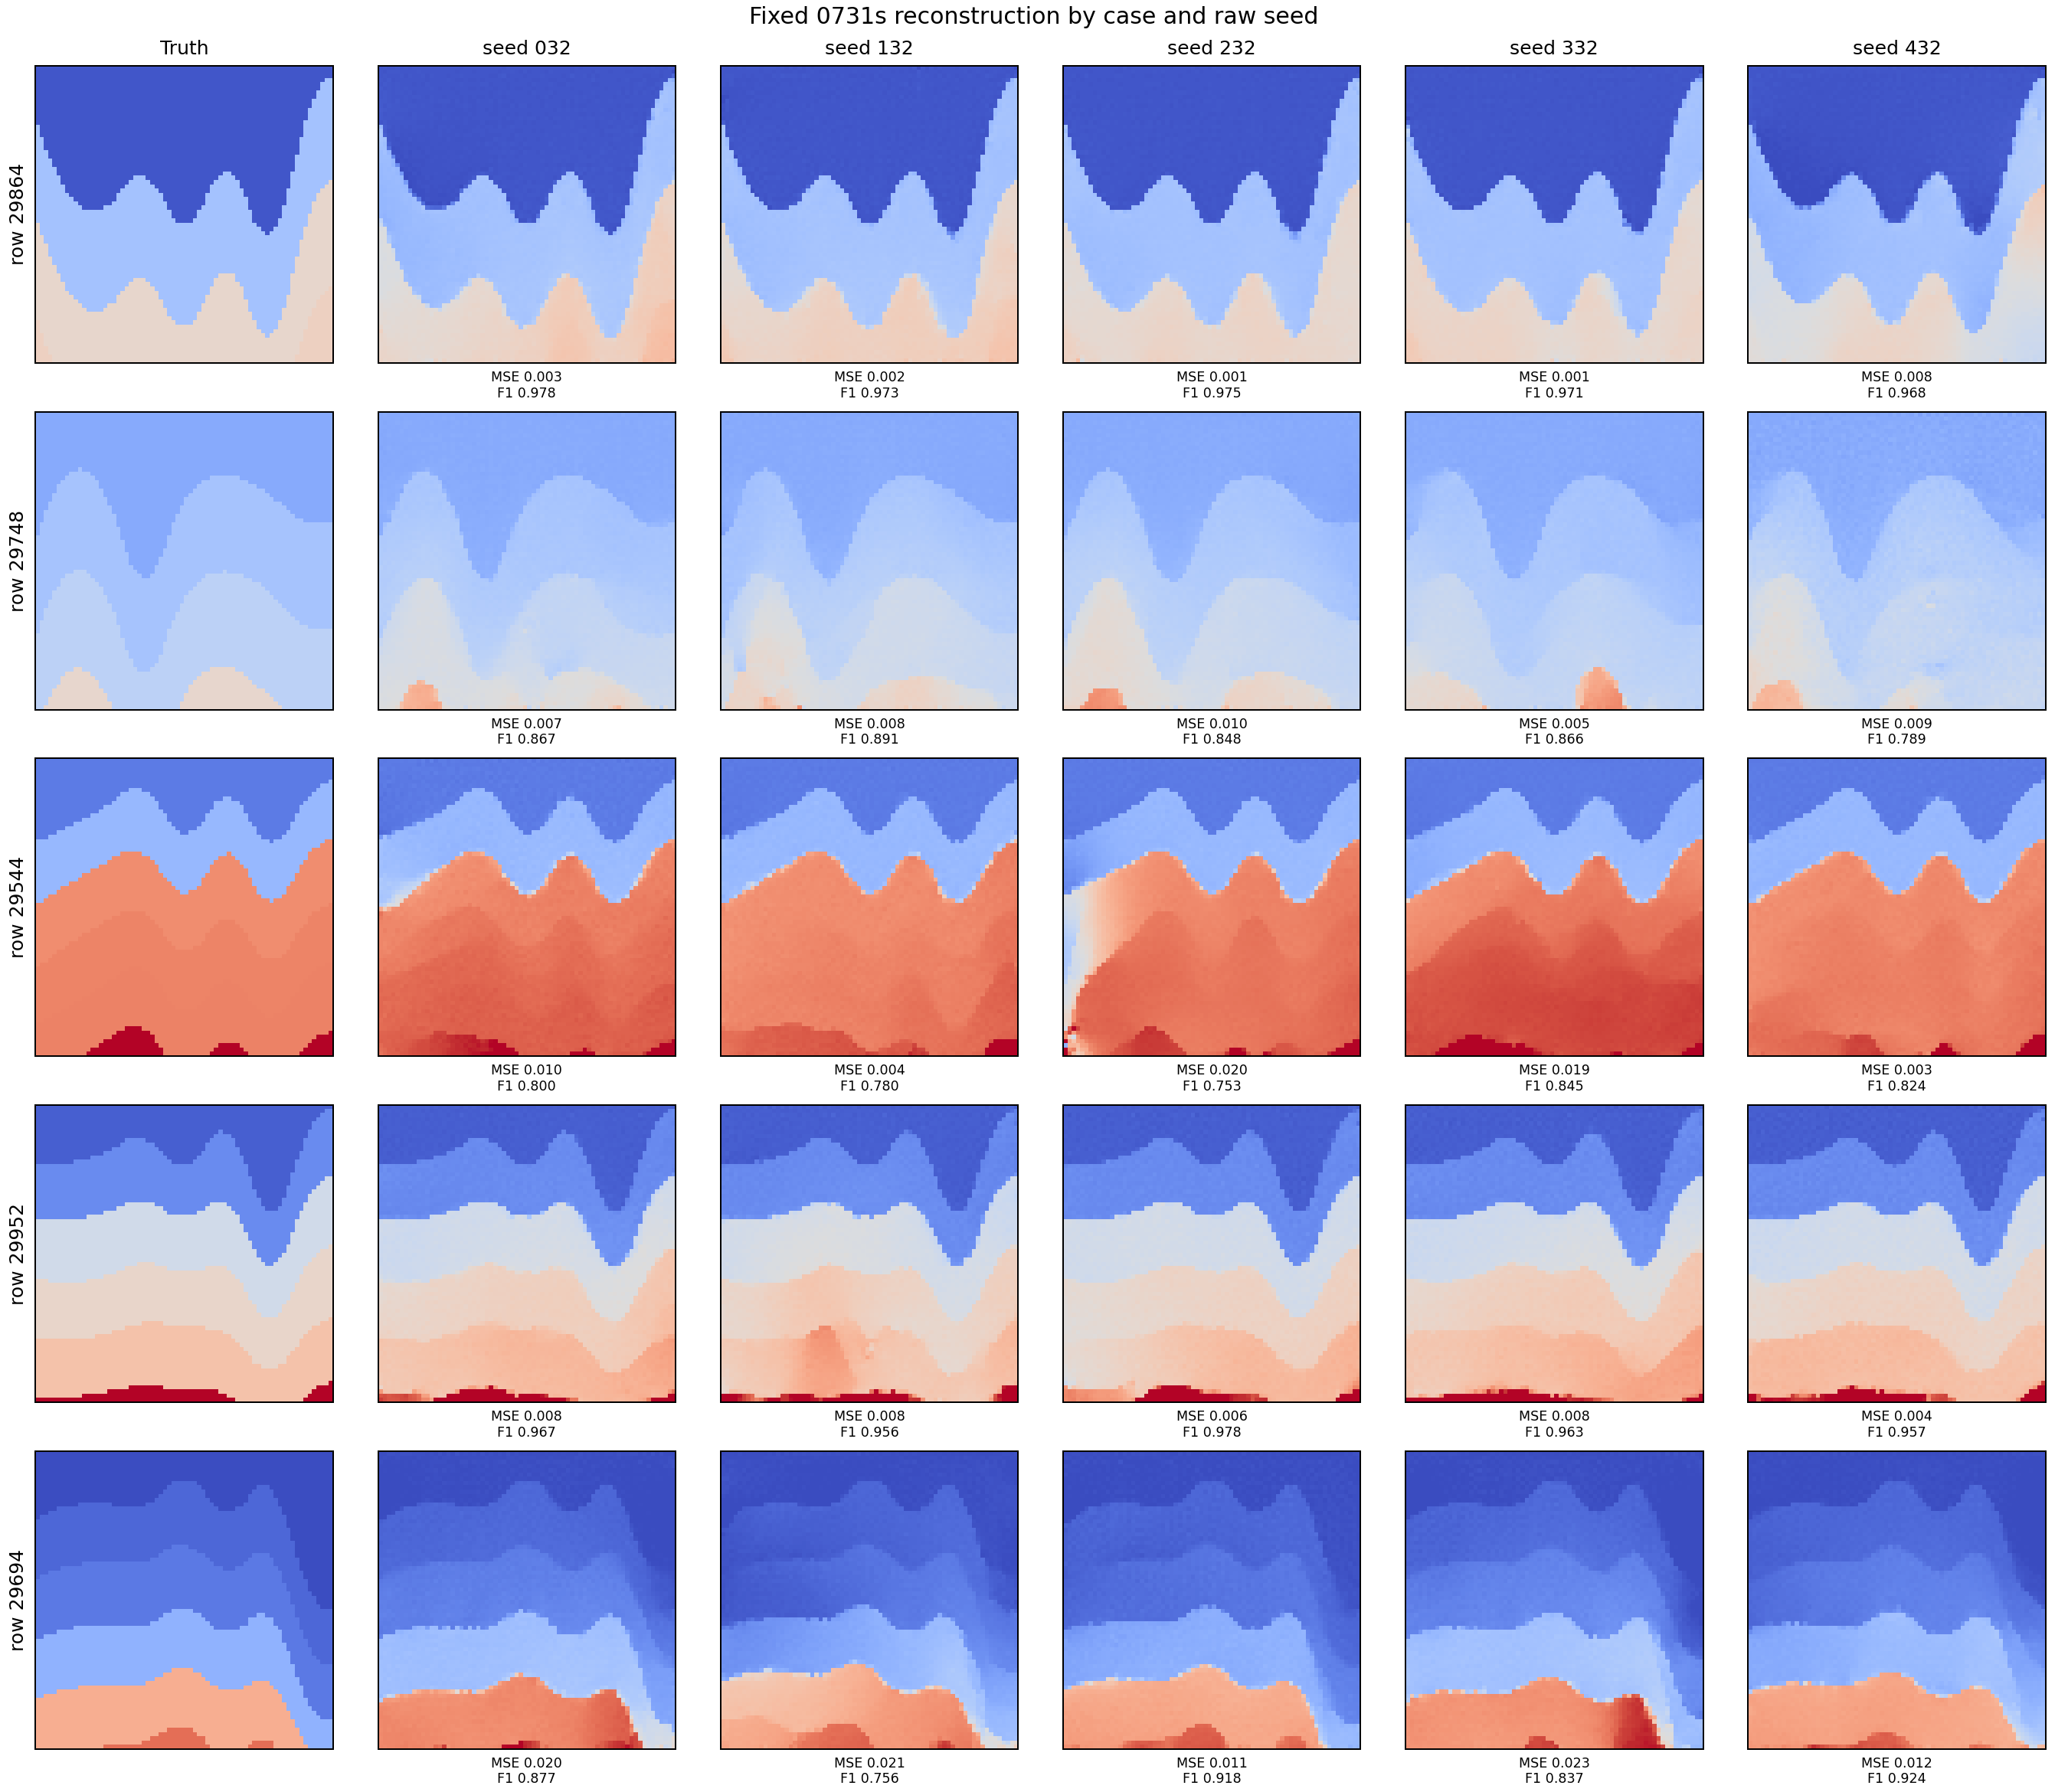
\includegraphics[width=\columnwidth]{../assets/figures/multiseed_models.png}
\caption{Truth and final reconstructions for five evaluation cases crossed with five prespecified raw seeds. Unlike Figure~\ref{fig:comparison}'s explicit row-oracle summary, this panel shows every run.}
\label{fig:models}
\end{figure}

The final endpoints obtain mean/maximum-observed MSE $0.00929/0.02305$ and mean/minimum boundary F1 $0.8905/0.7526$. Mean runtime is 2,978 seconds per cell. The unit of task variation is the geological case ($n=5$); seeds are repeated runs within case. We therefore report the complete crossed panel and paired cell-wise attribution descriptively, without treating the 25 cells as independent samples or claiming population-level significance.

Relative to the internal source stage, the final endpoint reduces mean MSE from $0.01424$ to $0.00929$ and the maximum observed MSE from $0.03219$ to $0.02305$. It improves MSE in 19/25 cells and boundary F1 in 22/25. These are descriptive within-pipeline comparisons: the source stage is not a compute-matched independent baseline, and a source off/on $\times$ Multi-Back off/on experiment is still needed to identify a causal interaction.

\subsection{Seed-sensitive source failures and Multi-Back rescue}
\begin{figure}[t]
\centering
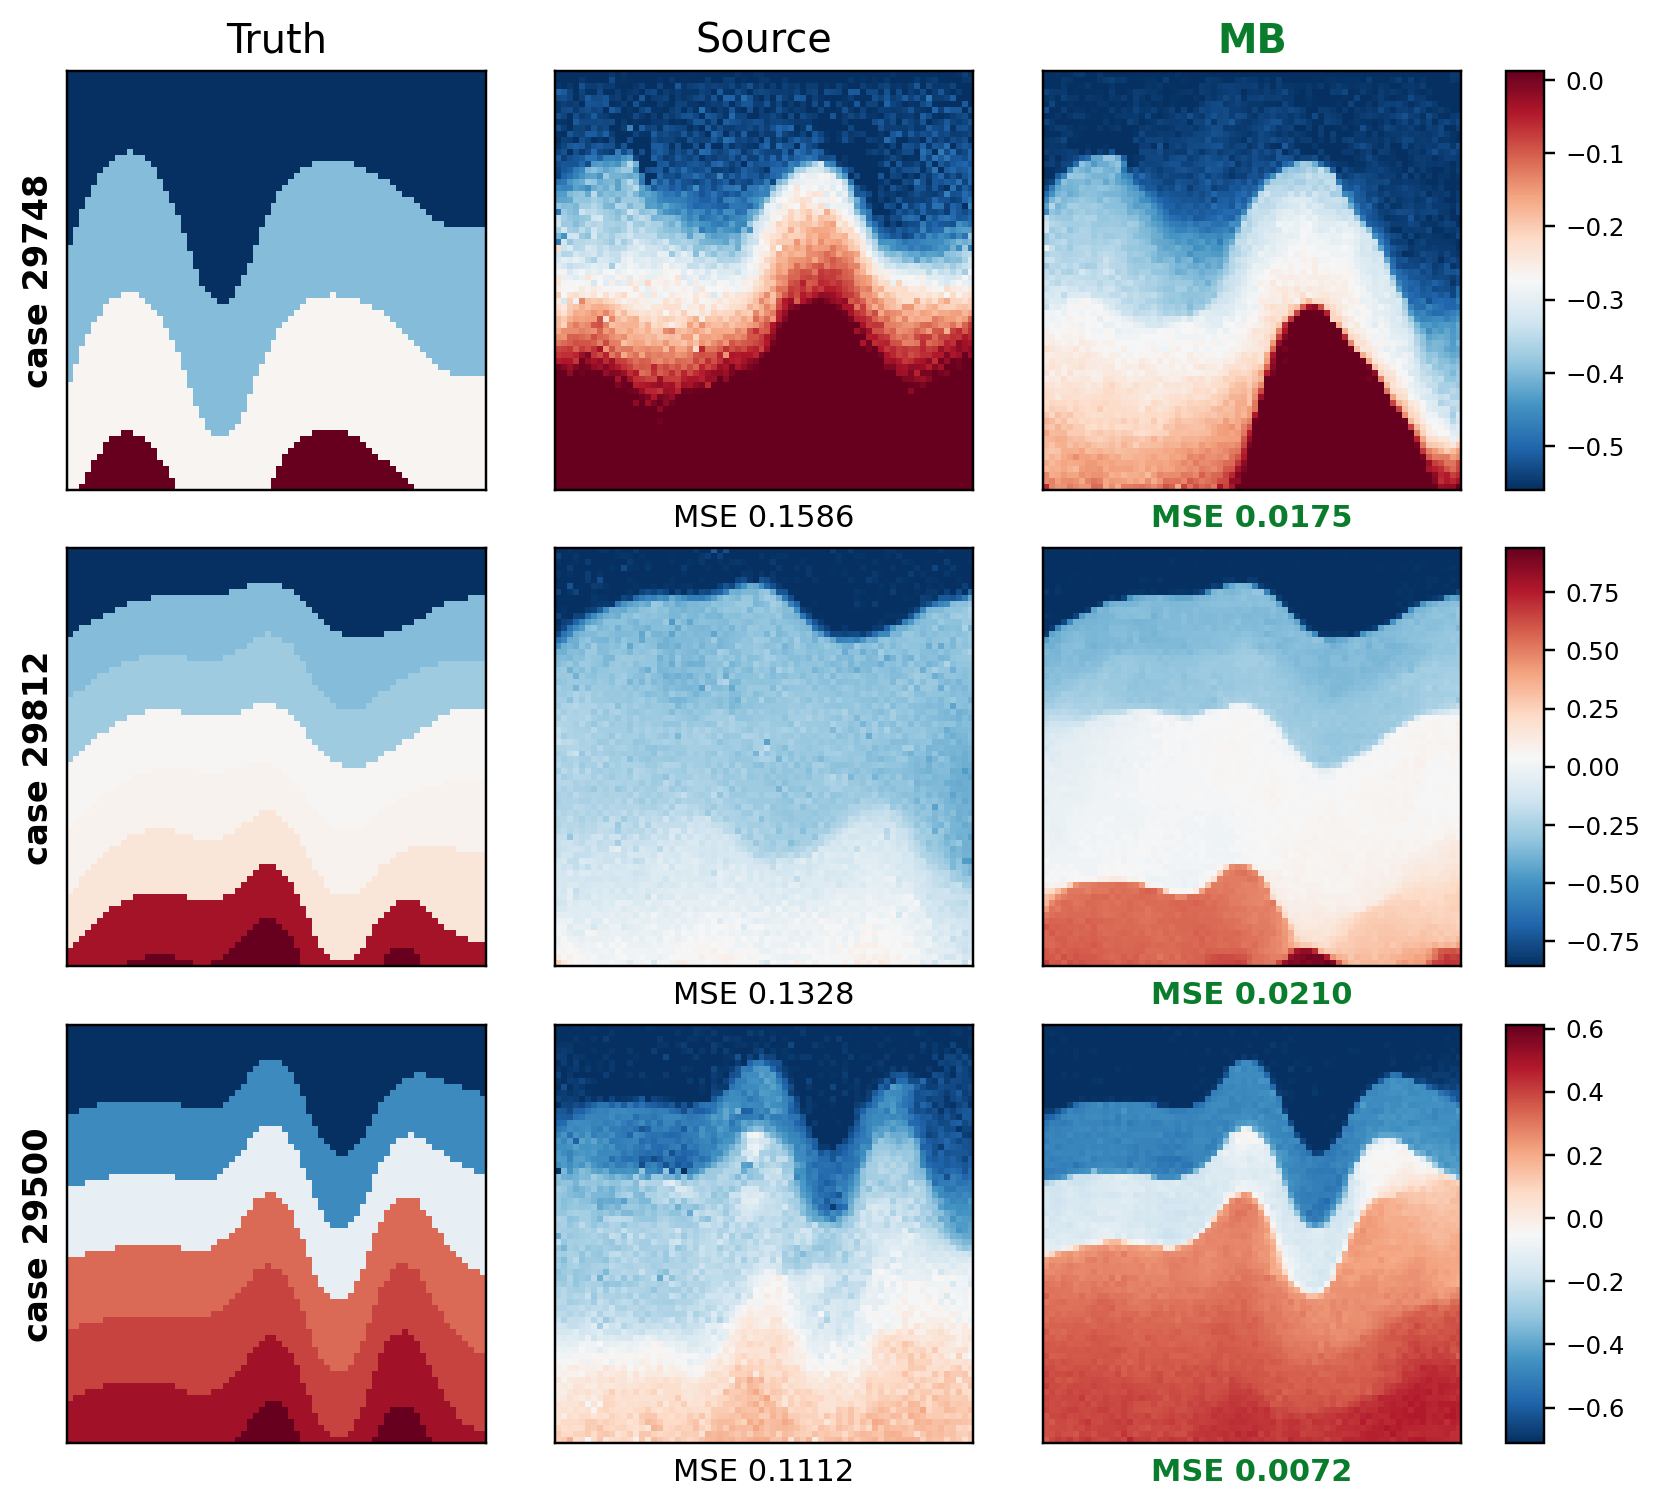
\includegraphics[width=\columnwidth]{../assets/figures/source_rescue.png}
\caption{Three catastrophic source cases and the corresponding Multi-Back recovery results.}
\label{fig:rescue}
\end{figure}

The rescue examples change MSE from $0.1586$ to $0.0175$, $0.1328$ to $0.0210$, and $0.1112$ to $0.0072$. They show that revisiting earlier generative times can repair a poor source reconstruction rather than merely sharpen an already correct interface.

\section{Limitations and Conclusion}
This study evaluates one synthetic acquisition family, five geological cases, and one frozen Flow Map prior. Across the frozen $5\times5$ panel, MBF obtains mean/maximum-observed MSE $0.00929/0.02305$ and mean/minimum boundary F1 $0.8905/0.7526$. Relative to the internal source stage, the final endpoint reduces mean MSE from $0.01424$ to $0.00929$, improving MSE in 19/25 cells and boundary F1 in 22/25 cells. These source-to-final comparisons are descriptive within the implemented pipeline and do not establish a causal source--Multi-Back interaction.

Within this scope, MBF reframes frozen generative inference as non-monotone control on a two-time flow graph. Flow Maps reduce the number of generative transitions, while Multi-Back introduces task-relevant directions from earlier generative scales. Matched external baselines, the prescribed factorial ablation, more independent cases, and validation on additional inverse operators are still required for broader causal or superiority claims.

\bibliographystyle{plain}
\bibliography{references}
\end{document}
